\documentclass{standalone}
\usepackage{tikz}
\usepackage{amsmath}
\usepackage{color}
\usetikzlibrary{matrix}
\usetikzlibrary {shapes.geometric}
\usetikzlibrary {math}
\usetikzlibrary {arrows.meta}

\begin{document}
        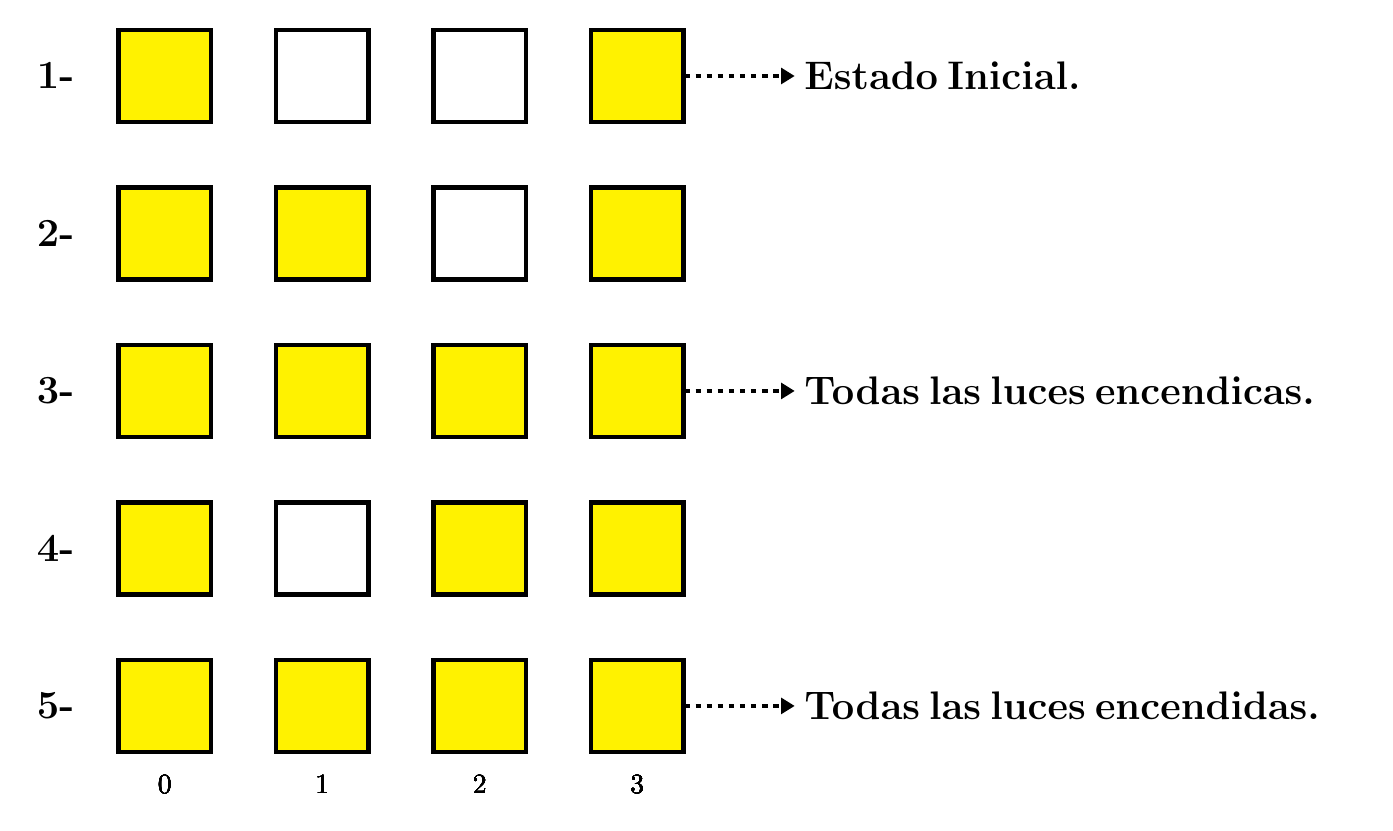
\begin{tikzpicture}
        %   \draw [help lines] (0,0) grid (16,16);
        \foreach \x/\y in {1,2,4,6,8/1,2,4,6,8,10}
        {
            \node [scale = 5,ultra thick,draw,fill = yellow] () at (2,10) {};
            \node [scale = 5,ultra thick,draw,] () at (4,10) {};
            \node [scale = 5,ultra thick,draw,] () at (6,10) {};
            \node [scale = 5,ultra thick,draw,fill = yellow] () at (8,10) {};

            \node [scale = 5,ultra thick,draw,fill = yellow] () at (2,8) {};
            \node [scale = 5,ultra thick,draw,fill = yellow] () at (4,8) {};
            \node [scale = 5,ultra thick,draw,] () at (6,8) {};
            \node [scale = 5,ultra thick,draw,fill = yellow] () at (8,8) {};

            \node [scale = 5,ultra thick,draw,fill = yellow] () at (2,6) {};
            \node [scale = 5,ultra thick,draw,fill = yellow] () at (4,6) {};
            \node [scale = 5,ultra thick,draw,fill = yellow] () at (6,6) {};
            \node [scale = 5,ultra thick,draw,fill = yellow] () at (8,6) {};

            \node [scale = 5,ultra thick,draw,fill = yellow] () at (2,4) {};
            \node [scale = 5,ultra thick,draw,] () at (4,4) {};
            \node [scale = 5,ultra thick,draw,fill = yellow] () at (6,4) {};
            \node [scale = 5,ultra thick,draw,fill = yellow] () at (8,4) {};

            \node [scale = 5,ultra thick,draw,fill = yellow] () at (2,2) {};
            \node [scale = 5,ultra thick,draw,fill = yellow] () at (4,2) {};
            \node [scale = 5,ultra thick,draw,fill = yellow] () at (6,2) {};
            \node [scale = 5,ultra thick,draw,fill = yellow] () at (8,2) {};

            \node at (2,1) {0};
            \node at (4,1) {1};
            \node at (6,1) {2};
            \node at (8,1) {3};
        }

        \draw[ultra thick,arrows = -{Triangle[open, angle=60:2mm,fill=black]}] [dash pattern=on 2pt off 2pt](8.6,10) -- (10,10);
        \draw[ultra thick,arrows = -{Triangle[open, angle=60:2mm,fill=black]}] [dash pattern=on 2pt off 2pt](8.6,6) -- (10,6);
        \draw[ultra thick,arrows = -{Triangle[open, angle=60:2mm,fill=black]}] [dash pattern=on 2pt off 2pt](8.6,2) -- (10,2);   
       
        \node [right=2cm,text width=5cm] at (8,10)
        {
        \mbox{\Large \textbf {Estado Inicial.}}
        };

        \node [right=2cm,text width=7cm] at (8,6)
        {
        \mbox{\Large \textbf {Todas las luces encendicas.}}
        };

        \node [right=2cm,text width=7cm] at (8,2)
        {
        \mbox{\Large \textbf {Todas las luces encendidas.}}
        };





        \node [left=0.1cm,text width=1.4cm] at (2,2)
        {
        \mbox{\Large \textbf {5-}}
        };

        \node [left=0.1cm,text width=1.4cm] at (2,4)
        {
        \mbox{\Large \textbf {4-}}
        };

        \node [left=0.1cm,text width=1.4cm] at (2,6)
        {
        \mbox{\Large \textbf {3-}}
        };

        \node [left=0.1cm,text width=1.4cm] at (2,8)
        {
        \mbox{\Large \textbf {2-}}
        };
        
        \node [left=0.1cm,text width=1.4cm] at (2,10)
        {
        \mbox{\Large \textbf {1-}}
        };
    \end{tikzpicture}
\end{document}